%%
% Copyright (c) 2017 - 2024, Pascal Wagler;
% Copyright (c) 2014 - 2024, John MacFarlane
%
% All rights reserved.
%
% Redistribution and use in source and binary forms, with or without
% modification, are permitted provided that the following conditions
% are met:
%
% - Redistributions of source code must retain the above copyright
% notice, this list of conditions and the following disclaimer.
%
% - Redistributions in binary form must reproduce the above copyright
% notice, this list of conditions and the following disclaimer in the
% documentation and/or other materials provided with the distribution.
%
% - Neither the name of John MacFarlane nor the names of other
% contributors may be used to endorse or promote products derived
% from this software without specific prior written permission.
%
% THIS SOFTWARE IS PROVIDED BY THE COPYRIGHT HOLDERS AND CONTRIBUTORS
% "AS IS" AND ANY EXPRESS OR IMPLIED WARRANTIES, INCLUDING, BUT NOT
% LIMITED TO, THE IMPLIED WARRANTIES OF MERCHANTABILITY AND FITNESS
% FOR A PARTICULAR PURPOSE ARE DISCLAIMED. IN NO EVENT SHALL THE
% COPYRIGHT OWNER OR CONTRIBUTORS BE LIABLE FOR ANY DIRECT, INDIRECT,
% INCIDENTAL, SPECIAL, EXEMPLARY, OR CONSEQUENTIAL DAMAGES (INCLUDING,
% BUT NOT LIMITED TO, PROCUREMENT OF SUBSTITUTE GOODS OR SERVICES;
% LOSS OF USE, DATA, OR PROFITS; OR BUSINESS INTERRUPTION) HOWEVER
% CAUSED AND ON ANY THEORY OF LIABILITY, WHETHER IN CONTRACT, STRICT
% LIABILITY, OR TORT (INCLUDING NEGLIGENCE OR OTHERWISE) ARISING IN
% ANY WAY OUT OF THE USE OF THIS SOFTWARE, EVEN IF ADVISED OF THE
% POSSIBILITY OF SUCH DAMAGE.
%%

%%
% This is the Eisvogel pandoc LaTeX template.
%
% For usage information and examples visit the official GitHub page:
% https://github.com/Wandmalfarbe/pandoc-latex-template
%%

% Options for packages loaded elsewhere
\PassOptionsToPackage{unicode}{hyperref}
\PassOptionsToPackage{hyphens}{url}
\PassOptionsToPackage{dvipsnames,svgnames,x11names,table}{xcolor}
%
\documentclass[
  paper=a4,
  ,captions=tableheading
]{scrartcl}
\usepackage{amsmath,amssymb}
% Use setspace anyway because we change the default line spacing.
% The spacing is changed early to affect the titlepage and the TOC.
\usepackage{setspace}
\setstretch{1.2}
\usepackage{iftex}
\ifPDFTeX
  \usepackage[T1]{fontenc}
  \usepackage[utf8]{inputenc}
  \usepackage{textcomp} % provide euro and other symbols
\else % if luatex or xetex
  \usepackage{unicode-math} % this also loads fontspec
  \defaultfontfeatures{Scale=MatchLowercase}
  \defaultfontfeatures[\rmfamily]{Ligatures=TeX,Scale=1}
\fi
\usepackage{lmodern}
\ifPDFTeX\else
  % xetex/luatex font selection
\fi
% Use upquote if available, for straight quotes in verbatim environments
\IfFileExists{upquote.sty}{\usepackage{upquote}}{}
\IfFileExists{microtype.sty}{% use microtype if available
  \usepackage[]{microtype}
  \UseMicrotypeSet[protrusion]{basicmath} % disable protrusion for tt fonts
}{}
\makeatletter
\@ifundefined{KOMAClassName}{% if non-KOMA class
  \IfFileExists{parskip.sty}{%
    \usepackage{parskip}
  }{% else
    \setlength{\parindent}{0pt}
    \setlength{\parskip}{6pt plus 2pt minus 1pt}}
}{% if KOMA class
  \KOMAoptions{parskip=half}}
\makeatother
\usepackage{xcolor}
\definecolor{default-linkcolor}{HTML}{A50000}
\definecolor{default-filecolor}{HTML}{A50000}
\definecolor{default-citecolor}{HTML}{4077C0}
\definecolor{default-urlcolor}{HTML}{4077C0}
\usepackage[margin=2.5cm,includehead=true,includefoot=true,centering,]{geometry}
\usepackage{longtable,booktabs,array}
\usepackage{calc} % for calculating minipage widths
% Correct order of tables after \paragraph or \subparagraph
\usepackage{etoolbox}
\makeatletter
\patchcmd\longtable{\par}{\if@noskipsec\mbox{}\fi\par}{}{}
\makeatother
% Allow footnotes in longtable head/foot
\IfFileExists{footnotehyper.sty}{\usepackage{footnotehyper}}{\usepackage{footnote}}
\makesavenoteenv{longtable}
% add backlinks to footnote references, cf. https://tex.stackexchange.com/questions/302266/make-footnote-clickable-both-ways
\usepackage{footnotebackref}
\usepackage{graphicx}
\makeatletter
\newsavebox\pandoc@box
\newcommand*\pandocbounded[1]{% scales image to fit in text height/width
  \sbox\pandoc@box{#1}%
  \Gscale@div\@tempa{\textheight}{\dimexpr\ht\pandoc@box+\dp\pandoc@box\relax}%
  \Gscale@div\@tempb{\linewidth}{\wd\pandoc@box}%
  \ifdim\@tempb\p@<\@tempa\p@\let\@tempa\@tempb\fi% select the smaller of both
  \ifdim\@tempa\p@<\p@\scalebox{\@tempa}{\usebox\pandoc@box}%
  \else\usebox{\pandoc@box}%
  \fi%
}
% Set default figure placement to htbp
% Make use of float-package and set default placement for figures to H.
% The option H means 'PUT IT HERE' (as  opposed to the standard h option which means 'You may put it here if you like').
\usepackage{float}
\floatplacement{figure}{H}
\makeatother
\setlength{\emergencystretch}{3em} % prevent overfull lines
\providecommand{\tightlist}{%
  \setlength{\itemsep}{0pt}\setlength{\parskip}{0pt}}
\setcounter{secnumdepth}{-\maxdimen} % remove section numbering
\ifLuaTeX
\usepackage[bidi=basic]{babel}
\else
\usepackage[bidi=default]{babel}
\fi
\babelprovide[main,import]{english}
% get rid of language-specific shorthands (see #6817):
\let\LanguageShortHands\languageshorthands
\def\languageshorthands#1{}
\makeatletter
\@ifpackageloaded{subfig}{}{\usepackage{subfig}}
\@ifpackageloaded{caption}{}{\usepackage{caption}}
\captionsetup[subfloat]{margin=0.5em}
\AtBeginDocument{%
\renewcommand*\figurename{Figura}
\renewcommand*\tablename{Tabla}
}
\AtBeginDocument{%
\renewcommand*\listfigurename{Lista de Figuras}
\renewcommand*\listtablename{Lista de Tablas}
}
\newcounter{pandoccrossref@subfigures@footnote@counter}
\newenvironment{pandoccrossrefsubfigures}{%
\setcounter{pandoccrossref@subfigures@footnote@counter}{0}
\begin{figure}\centering%
\gdef\global@pandoccrossref@subfigures@footnotes{}%
\DeclareRobustCommand{\footnote}[1]{\footnotemark%
\stepcounter{pandoccrossref@subfigures@footnote@counter}%
\ifx\global@pandoccrossref@subfigures@footnotes\empty%
\gdef\global@pandoccrossref@subfigures@footnotes{{##1}}%
\else%
\g@addto@macro\global@pandoccrossref@subfigures@footnotes{, {##1}}%
\fi}}%
{\end{figure}%
\addtocounter{footnote}{-\value{pandoccrossref@subfigures@footnote@counter}}
\@for\f:=\global@pandoccrossref@subfigures@footnotes\do{\stepcounter{footnote}\footnotetext{\f}}%
\gdef\global@pandoccrossref@subfigures@footnotes{}}
\@ifpackageloaded{float}{}{\usepackage{float}}
\floatstyle{ruled}
\@ifundefined{c@chapter}{\newfloat{codelisting}{h}{lop}}{\newfloat{codelisting}{h}{lop}[chapter]}
\floatname{codelisting}{Listing}
\newcommand*\listoflistings{\listof{codelisting}{Listas del Documento}}
\makeatother
\usepackage{bookmark}
\IfFileExists{xurl.sty}{\usepackage{xurl}}{} % add URL line breaks if available
\urlstyle{same}
\hypersetup{
  pdftitle={Vinaque sanguine metuenti cuiquam Alcyone fixus},
  pdfauthor={Author Name},
  pdflang={en},
  pdfsubject={Markdown},
  pdfkeywords={Markdown, Example},
  hidelinks,
  breaklinks=true,
  pdfcreator={LaTeX via pandoc with the Eisvogel template}}
\title{Vinaque sanguine metuenti cuiquam Alcyone fixus}
\usepackage{etoolbox}
\makeatletter
\providecommand{\subtitle}[1]{% add subtitle to \maketitle
  \apptocmd{\@title}{\par {\large #1 \par}}{}{}
}
\makeatother
\subtitle{Aesculeae domus vincemur et Veneris adsuetus lapsum}
\author{Author Name}
\date{2017-02-20}



%%
%% added
%%


%
% for the background color of the title page
%
\usepackage{pagecolor}
\usepackage{afterpage}
\usepackage{tikz}
\usepackage[margin=2.5cm,includehead=true,includefoot=true,centering]{geometry}

%
% break urls
%
\PassOptionsToPackage{hyphens}{url}

%
% When using babel or polyglossia with biblatex, loading csquotes is recommended
% to ensure that quoted texts are typeset according to the rules of your main language.
%
\usepackage{csquotes}

%
% captions
%
\definecolor{caption-color}{HTML}{777777}
\usepackage[font={stretch=1.2}, textfont={color=caption-color}, position=top, skip=4mm, labelfont=bf, singlelinecheck=false, justification=raggedright]{caption}
\setcapindent{0em}

%
% blockquote
%
\definecolor{blockquote-border}{RGB}{221,221,221}
\definecolor{blockquote-text}{RGB}{119,119,119}
\usepackage{mdframed}
\newmdenv[rightline=false,bottomline=false,topline=false,linewidth=3pt,linecolor=blockquote-border,skipabove=\parskip]{customblockquote}
\renewenvironment{quote}{\begin{customblockquote}\list{}{\rightmargin=0em\leftmargin=0em}%
\item\relax\color{blockquote-text}\ignorespaces}{\unskip\unskip\endlist\end{customblockquote}}

%
% Source Sans Pro as the default font family
% Source Code Pro for monospace text
%
% 'default' option sets the default
% font family to Source Sans Pro, not \sfdefault.
%
\ifnum 0\ifxetex 1\fi\ifluatex 1\fi=0 % if pdftex
    \usepackage[default]{sourcesanspro}
  \usepackage{sourcecodepro}
  \else % if not pdftex
    \usepackage[default]{sourcesanspro}
  \usepackage{sourcecodepro}

  % XeLaTeX specific adjustments for straight quotes: https://tex.stackexchange.com/a/354887
  % This issue is already fixed (see https://github.com/silkeh/latex-sourcecodepro/pull/5) but the
  % fix is still unreleased.
  % TODO: Remove this workaround when the new version of sourcecodepro is released on CTAN.
  \ifxetex
    \makeatletter
    \defaultfontfeatures[\ttfamily]
      { Numbers   = \sourcecodepro@figurestyle,
        Scale     = \SourceCodePro@scale,
        Extension = .otf }
    \setmonofont
      [ UprightFont    = *-\sourcecodepro@regstyle,
        ItalicFont     = *-\sourcecodepro@regstyle It,
        BoldFont       = *-\sourcecodepro@boldstyle,
        BoldItalicFont = *-\sourcecodepro@boldstyle It ]
      {SourceCodePro}
    \makeatother
  \fi
  \fi

%
% heading color
%
\definecolor{heading-color}{RGB}{40,40,40}
\addtokomafont{section}{\color{heading-color}}
% When using the classes report, scrreprt, book,
% scrbook or memoir, uncomment the following line.
%\addtokomafont{chapter}{\color{heading-color}}

%
% variables for title, author and date
%
\usepackage{titling}
\title{Vinaque sanguine metuenti cuiquam Alcyone fixus}
\author{Author Name}
\date{2017-02-20}

%
% tables
%

\definecolor{table-row-color}{HTML}{F5F5F5}
\definecolor{table-rule-color}{HTML}{999999}

%\arrayrulecolor{black!40}
\arrayrulecolor{table-rule-color}     % color of \toprule, \midrule, \bottomrule
\setlength\heavyrulewidth{0.3ex}      % thickness of \toprule, \bottomrule
\renewcommand{\arraystretch}{1.3}     % spacing (padding)


%
% remove paragraph indentation
%
\setlength{\parindent}{0pt}
\setlength{\parskip}{6pt plus 2pt minus 1pt}
\setlength{\emergencystretch}{3em}  % prevent overfull lines

%
%
% Listings
%
%


%
% header and footer
%
\usepackage[headsepline,footsepline]{scrlayer-scrpage}

\newpairofpagestyles{eisvogel-header-footer}{
  \clearpairofpagestyles
  \ihead*{Vinaque sanguine metuenti cuiquam Alcyone fixus}
  \chead*{}
  \ohead*{2017-02-20}
  \ifoot*{Author Name}
  \cfoot*{}
  \ofoot*{\thepage}
  \addtokomafont{pageheadfoot}{\upshape}
}
\pagestyle{eisvogel-header-footer}



%%
%% end added
%%

\begin{document}

%%
%% begin titlepage
%%
\begin{titlepage}
\newgeometry{top=2cm, right=4cm, bottom=3cm, left=4cm}
\tikz[remember picture,overlay] \node[inner sep=0pt] at (current page.center){
\includegraphics[width=\paperwidth,height=\paperheight]{background1.pdf}};
\newcommand{\colorRule}[3][black]{\textcolor[HTML]{#1}{\rule{#2}{#3}}}
\begin{flushleft}
\noindent
\\[-1em]
\color[HTML]{5F5F5F}
\makebox[0pt][l]{\colorRule[360049]{1.3\textwidth}{4pt}}
\par
\noindent

% The titlepage with a background image has other text spacing and text size
{
  \setstretch{2}
  \vfill
  \vskip -8em
  \noindent {\huge \textbf{\textsf{Vinaque sanguine metuenti cuiquam
Alcyone fixus}}}
    \vskip 1em
  {\Large \textsf{Aesculeae domus vincemur et Veneris adsuetus lapsum}}
    \vskip 2em
  \noindent {\Large \textsf{Author
Name} \vskip 0.6em \textsf{2017-02-20}}
  \vfill
}


\end{flushleft}
\end{titlepage}
\restoregeometry
\pagenumbering{arabic}

%%
%% end titlepage
%%

% \maketitle


Modelo de Integración. Proyecto JEP, 2024. Softgic.

Capacidades del modelo de integración para la impleentación de
requerimientos de interoperabilidad del proyecto Integración JEP, 2024.

04.ing.3n.Ver 0.2.33

\section{04.ING.3n.1. Modelo de Interoperabilidad JEP,
2024}\label{sec:ing.3n.1.-modelo-de-interoperabilidad-jep-2024}

\begin{itemize}
\tightlist
\item
  \hyperref[Introducciuxf3n]{Introducción}
\item
  \hyperref[entregables-grouping]{Entregables (Grouping)}

  \begin{itemize}
  \tightlist
  \item
    \hyperref[entg01.-soluciuxf3n-de-integraciuxf3n-jep-application-component]{ENTG01.
    Solución de Integración JEP (Application Component)}
  \item
    \hyperref[entg02.-servicios-de-integraciuxf3n-jep-application-service]{ENTG02.
    Servicios de Integración JEP (Application Service)}
  \item
    \hyperref[entg04.-nodo-integraciuxf3n-jep-node]{ENTG04. Nodo
    Integración JEP (Node)}

    \begin{itemize}
    \tightlist
    \item
      \hyperref[entg06.-contenedor-application-component]{ENTG06.
      Contenedor (Application Component)}

      \begin{itemize}
      \tightlist
      \item
        \hyperref[entg07-ltlttaskgtgt-application-service]{ENTG07
        \&lt;\&lt;task\&gt;\&gt; (Application Service)}
      \end{itemize}
    \item
      \hyperref[entg05.-proceso-ltltworkergtgt-application-process]{ENTG05.
      Proceso \&lt;\&lt;worker\&gt;\&gt; (Application Process)}
    \end{itemize}
  \item
    \hyperref[entg03.-cicd-integraciuxf3n-jep-technology-service]{ENTG03.
    CI/CD Integración JEP (Technology Service)}
  \item
    \hyperref[entg04.-nodo-integraciuxf3n-jep-node-2]{ENTG04. Nodo
    Integración JEP (Node) 2}

    \begin{itemize}
    \tightlist
    \item
      \hyperref[entg06.-contenedor-application-component-2]{ENTG06.
      Contenedor (Application Component) 2}

      \begin{itemize}
      \tightlist
      \item
        \hyperref[entg07-ltlttaskgtgt-application-service-2]{ENTG07
        \&lt;\&lt;task\&gt;\&gt; (Application Service) 2}
      \end{itemize}
    \item
      \hyperref[entg05.-proceso-ltltworkergtgt-application-process-2]{ENTG05.
      Proceso \&lt;\&lt;worker\&gt;\&gt; (Application Process) 2}
    \end{itemize}
  \end{itemize}
\item
  \hyperref[gestiuxf3n-integraciuxf3n-grouping]{Gestión Integración
  (Grouping)}

  \begin{itemize}
  \tightlist
  \item
    \hyperref[monitoreo-de-ssrvc-integraciuxf3n-constraint]{Monitoreo de
    (ssrvc) integración (Constraint)}
  \item
    \hyperref[requerimientos-integraciuxf3n-jep-requirement]{Requerimientos
    integración JEP (Requirement)}
  \item
    \hyperref[alcance-proyecto-integraciuxf3n-goal]{Alcance Proyecto
    Integración (Goal)}
  \item
    \hyperref[justificaciuxf3n-proyecto-integraciuxf3n-jep-driver]{Justificación
    Proyecto Integración JEP (Driver)}
  \item
    \hyperref[objeto-contractual-proyecto-jep-principle]{Objeto
    Contractual Proyecto JEP (Principle)}
  \item
    \hyperref[uso-de-infraestrucutra-tecnoluxf3gica-jep-constraint]{Uso
    de Infraestrucutra Tecnológica JEP (Constraint)}
  \end{itemize}
\item
  \hyperref[modelo-de-integraciuxf3n-jepux2c-2024.-softgic-grouping]{Modelo
  de Integración JEP, 2024. Softgic (Grouping)}

  \begin{itemize}
  \tightlist
  \item
    \hyperref[transporte-capability]{Transporte (Capability)}
  \item
    \hyperref[plano-de-administraciuxf3n-capability]{Plano de
    Administración (Capability)}
  \item
    \hyperref[esquema-de-datos-capability]{Esquema de Datos
    (Capability)}
  \item
    \hyperref[transformaciuxf3n-de-mensajes-capability]{Transformación
    de Mensajes (Capability)}
  \item
    \hyperref[modelo-de-seguridad-capability]{Modelo de Seguridad
    (Capability)}
  \item
    \hyperref[condiciones-de-despliegue-capability]{Condiciones de
    Despliegue (Capability)}
  \item
    \hyperref[composiciuxf3n-de-servicios-capability]{Composición de
    Servicios (Capability)}
  \item
    \hyperref[proveedores-y-consumidores-capability]{Proveedores y
    Consumidores (Capability)}
  \item
    \hyperref[alcance-de-la-integraciuxf3n-capability]{Alcance de la
    Integración (Capability)}
  \item
    \hyperref[tecnologuxedas-capability]{Tecnologías (Capability)}
  \item
    \hyperref[conectividad-api-capability]{Conectividad API
    (Capability)}
  \item
    \hyperref[contratos-de-interoperabilidad-capability]{Contratos de
    Interoperabilidad (Capability)}
  \item
    \hyperref[tipo-de-comunicaciuxf3n-capability]{Tipo de Comunicación
    (Capability)}
  \item
    \hyperref[sistema-de-mensajes-capability]{Sistema de Mensajes
    (Capability)}
  \item
    \hyperref[patruxf3n-de-integraciuxf3n-eip-capability]{Patrón de
    Integración (EIP) (Capability)}
  \item
    \hyperref[integraciuxf3n-de-procesos-capability]{Integración de
    Procesos (Capability)}
  \item
    \hyperref[flujo-de-datos-capability]{Flujo de datos (Capability)}
  \item
    \hyperref[soluciuxf3n-de-integraciuxf3n-capability]{Solución de
    Integración (Capability)}
  \item
    \hyperref[ambientes-y-herramientas-capability]{Ambientes y
    Herramientas (Capability)}
  \end{itemize}
\end{itemize}

\subsection{Introducción}\label{sec:introducciuxf3n}

\begin{figure}
\centering
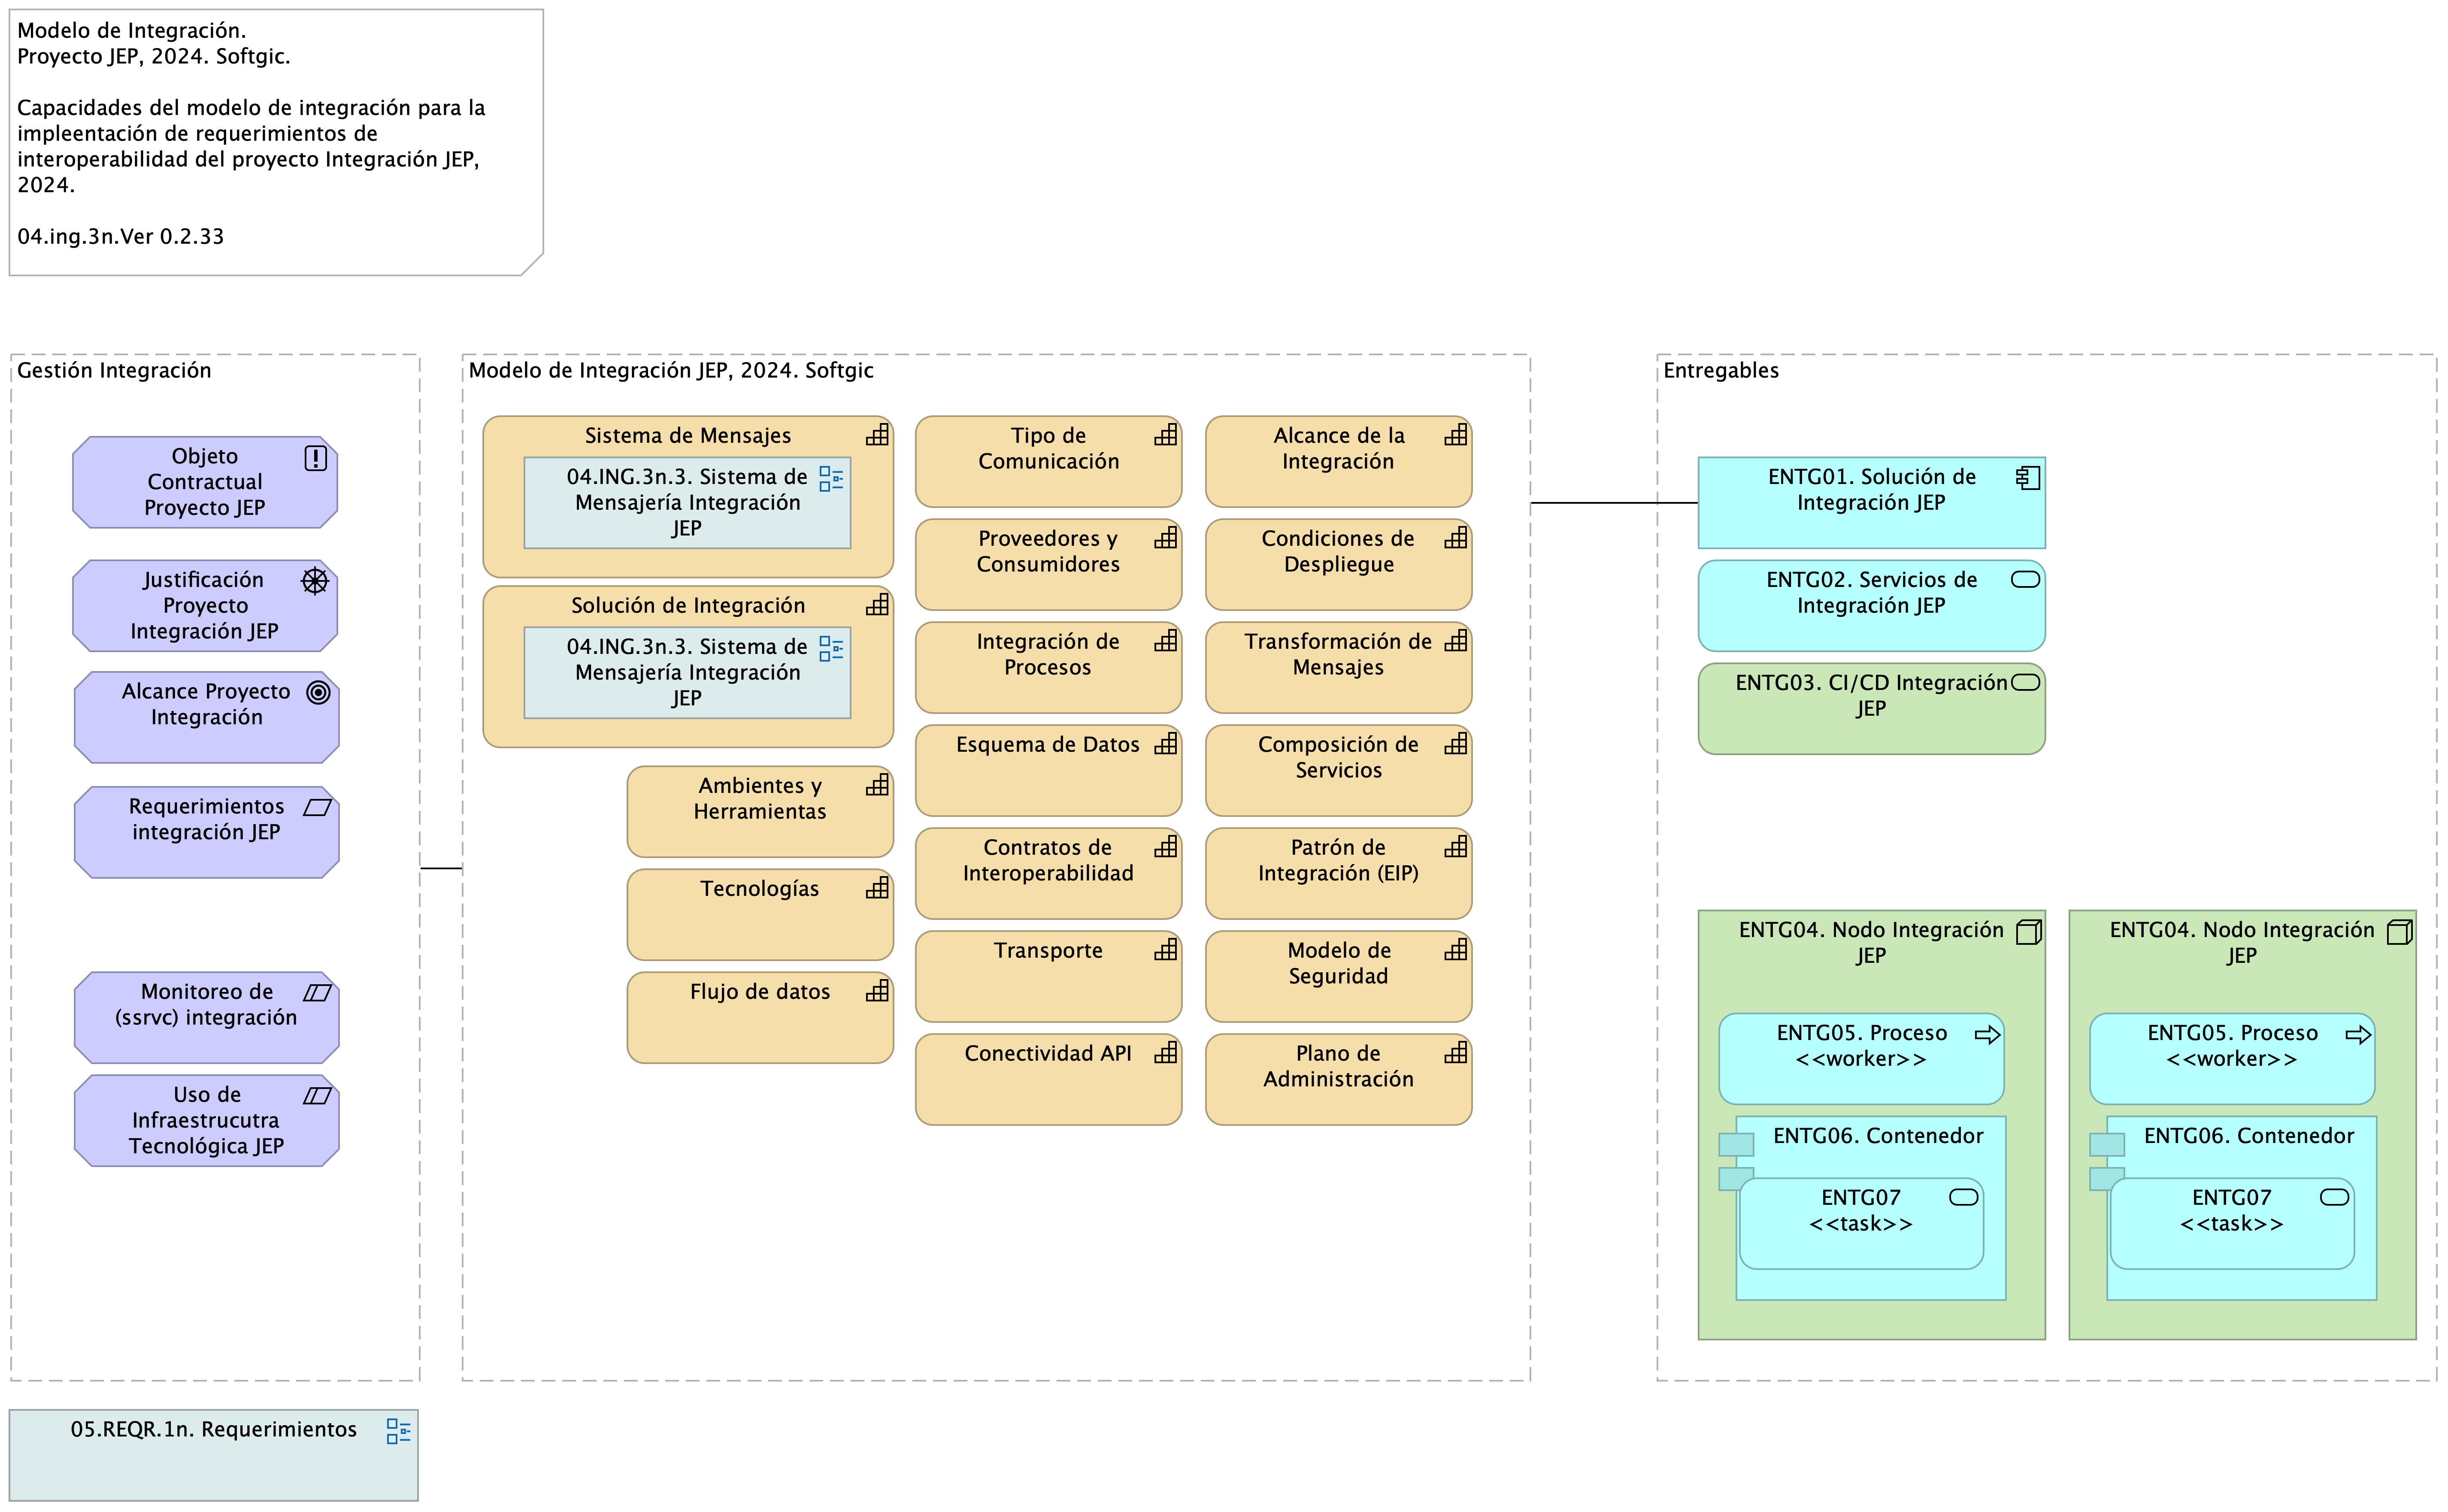
\includegraphics{01.1n.modelointegrac.png}
\caption{04.ING.3n.1. Modelo de Interoperabilidad JEP, 2024}
\end{figure}

El presente modelo de solución de interoperabilidad JEP, 2024, en
desarrollo por Softgic, expone para aprobación y referencia las
decisiones de la solución de integración y las restricciones que la
rigen. Una vez revisado y aprobado por parte de JEP el modelo de
interoperabilidad será referencia para la gestión del proyecto y de los
entregables de esta solución.

\subsection{Características Principales del Modelo de Integración
JEP}\label{sec:caracteruxedsticas-principales-del-modelo-de-integraciuxf3n-jep}

\begin{itemize}
\tightlist
\item
  API de integración
\item
  Patrones de integración empresarial (EIP)
\item
  Sistema de Mensajería entre servicios de integración y aplicaciones
  JEP
\item
  Flujos de datos para integración
\item
  Arquitectura de clusters y contenedores para integración
\item
  Uso de infraestructura tecnológica JEP
\end{itemize}

Versión fcb28c6 - cfg--restore - Fri, 25 Oct 2024 13:15:18 -0500

Modelo de Integración. Proyecto JEP, 2024. Softgic.

Capacidades del modelo de integración para la impleentación de
requerimientos de interoperabilidad del proyecto Integración JEP, 2024.

04.ing.3n.Ver 0.2.33

\section{04.ING.3n.1. Modelo de Interoperabilidad JEP,
2024}\label{sec:ing.3n.1.-modelo-de-interoperabilidad-jep-2024-1}

\begin{itemize}
\tightlist
\item
  \hyperref[Introducciuxf3n]{Introducción}
\item
  \hyperref[entregables-grouping]{Entregables (Grouping)}

  \begin{itemize}
  \tightlist
  \item
    \hyperref[entg01.-soluciuxf3n-de-integraciuxf3n-jep-application-component]{ENTG01.
    Solución de Integración JEP (Application Component)}
  \item
    \hyperref[entg02.-servicios-de-integraciuxf3n-jep-application-service]{ENTG02.
    Servicios de Integración JEP (Application Service)}
  \item
    \hyperref[entg04.-nodo-integraciuxf3n-jep-node]{ENTG04. Nodo
    Integración JEP (Node)}

    \begin{itemize}
    \tightlist
    \item
      \hyperref[entg06.-contenedor-application-component]{ENTG06.
      Contenedor (Application Component)}

      \begin{itemize}
      \tightlist
      \item
        \hyperref[entg07-ltlttaskgtgt-application-service]{ENTG07
        \&lt;\&lt;task\&gt;\&gt; (Application Service)}
      \end{itemize}
    \item
      \hyperref[entg05.-proceso-ltltworkergtgt-application-process]{ENTG05.
      Proceso \&lt;\&lt;worker\&gt;\&gt; (Application Process)}
    \end{itemize}
  \item
    \hyperref[entg03.-cicd-integraciuxf3n-jep-technology-service]{ENTG03.
    CI/CD Integración JEP (Technology Service)}
  \item
    \hyperref[entg04.-nodo-integraciuxf3n-jep-node-2]{ENTG04. Nodo
    Integración JEP (Node) 2}

    \begin{itemize}
    \tightlist
    \item
      \hyperref[entg06.-contenedor-application-component-2]{ENTG06.
      Contenedor (Application Component) 2}

      \begin{itemize}
      \tightlist
      \item
        \hyperref[entg07-ltlttaskgtgt-application-service-2]{ENTG07
        \&lt;\&lt;task\&gt;\&gt; (Application Service) 2}
      \end{itemize}
    \item
      \hyperref[entg05.-proceso-ltltworkergtgt-application-process-2]{ENTG05.
      Proceso \&lt;\&lt;worker\&gt;\&gt; (Application Process) 2}
    \end{itemize}
  \end{itemize}
\item
  \hyperref[gestiuxf3n-integraciuxf3n-grouping]{Gestión Integración
  (Grouping)}

  \begin{itemize}
  \tightlist
  \item
    \hyperref[monitoreo-de-ssrvc-integraciuxf3n-constraint]{Monitoreo de
    (ssrvc) integración (Constraint)}
  \item
    \hyperref[requerimientos-integraciuxf3n-jep-requirement]{Requerimientos
    integración JEP (Requirement)}
  \item
    \hyperref[alcance-proyecto-integraciuxf3n-goal]{Alcance Proyecto
    Integración (Goal)}
  \item
    \hyperref[justificaciuxf3n-proyecto-integraciuxf3n-jep-driver]{Justificación
    Proyecto Integración JEP (Driver)}
  \item
    \hyperref[objeto-contractual-proyecto-jep-principle]{Objeto
    Contractual Proyecto JEP (Principle)}
  \item
    \hyperref[uso-de-infraestrucutra-tecnoluxf3gica-jep-constraint]{Uso
    de Infraestrucutra Tecnológica JEP (Constraint)}
  \end{itemize}
\item
  \hyperref[modelo-de-integraciuxf3n-jepux2c-2024.-softgic-grouping]{Modelo
  de Integración JEP, 2024. Softgic (Grouping)}

  \begin{itemize}
  \tightlist
  \item
    \hyperref[transporte-capability]{Transporte (Capability)}
  \item
    \hyperref[plano-de-administraciuxf3n-capability]{Plano de
    Administración (Capability)}
  \item
    \hyperref[esquema-de-datos-capability]{Esquema de Datos
    (Capability)}
  \item
    \hyperref[transformaciuxf3n-de-mensajes-capability]{Transformación
    de Mensajes (Capability)}
  \item
    \hyperref[modelo-de-seguridad-capability]{Modelo de Seguridad
    (Capability)}
  \item
    \hyperref[condiciones-de-despliegue-capability]{Condiciones de
    Despliegue (Capability)}
  \item
    \hyperref[composiciuxf3n-de-servicios-capability]{Composición de
    Servicios (Capability)}
  \item
    \hyperref[proveedores-y-consumidores-capability]{Proveedores y
    Consumidores (Capability)}
  \item
    \hyperref[alcance-de-la-integraciuxf3n-capability]{Alcance de la
    Integración (Capability)}
  \item
    \hyperref[tecnologuxedas-capability]{Tecnologías (Capability)}
  \item
    \hyperref[conectividad-api-capability]{Conectividad API
    (Capability)}
  \item
    \hyperref[contratos-de-interoperabilidad-capability]{Contratos de
    Interoperabilidad (Capability)}
  \item
    \hyperref[tipo-de-comunicaciuxf3n-capability]{Tipo de Comunicación
    (Capability)}
  \item
    \hyperref[sistema-de-mensajes-capability]{Sistema de Mensajes
    (Capability)}
  \item
    \hyperref[patruxf3n-de-integraciuxf3n-eip-capability]{Patrón de
    Integración (EIP) (Capability)}
  \item
    \hyperref[integraciuxf3n-de-procesos-capability]{Integración de
    Procesos (Capability)}
  \item
    \hyperref[flujo-de-datos-capability]{Flujo de datos (Capability)}
  \item
    \hyperref[soluciuxf3n-de-integraciuxf3n-capability]{Solución de
    Integración (Capability)}
  \item
    \hyperref[ambientes-y-herramientas-capability]{Ambientes y
    Herramientas (Capability)}
  \end{itemize}
\end{itemize}

\subsection{Introducción}\label{sec:introducciuxf3n-1}

\begin{figure}
\centering
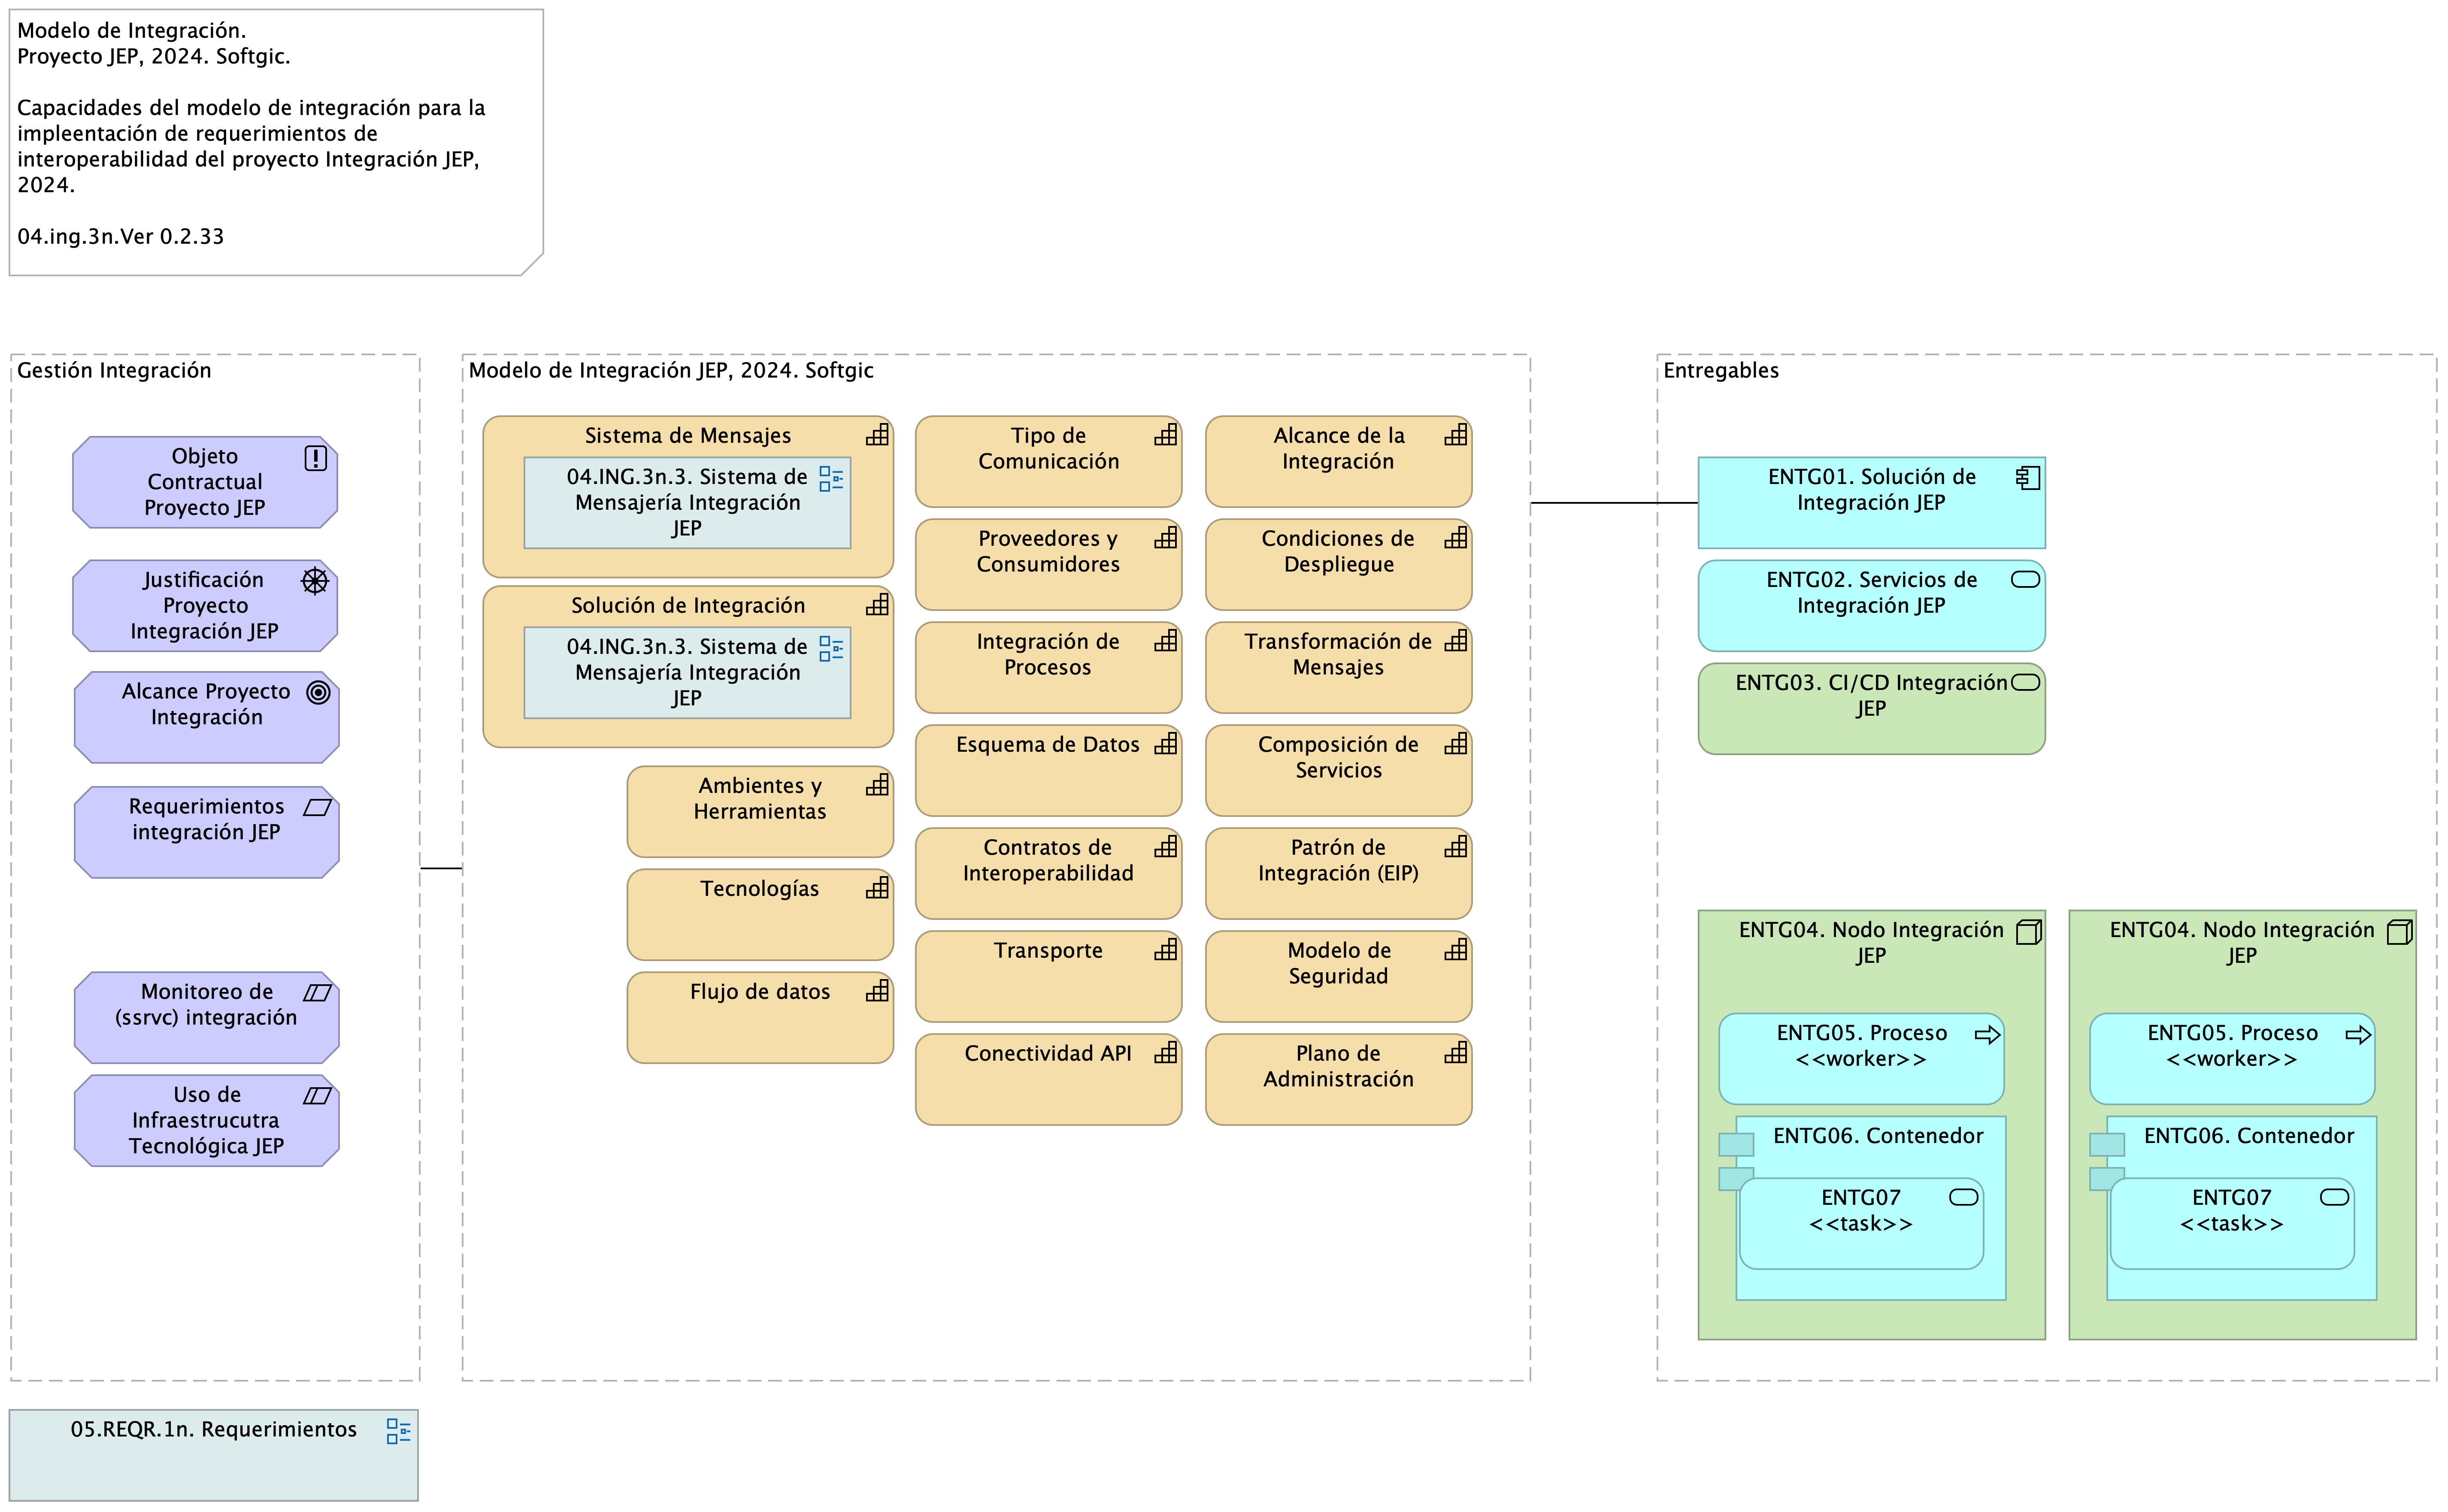
\includegraphics{01.1n.modelointegrac.png}
\caption{04.ING.3n.1. Modelo de Interoperabilidad JEP, 2024}
\end{figure}

El presente modelo de solución de interoperabilidad JEP, 2024, en
desarrollo por Softgic, expone para aprobación y referencia las
decisiones de la solución de integración y las restricciones que la
rigen. Una vez revisado y aprobado por parte de JEP el modelo de
interoperabilidad será referencia para la gestión del proyecto y de los
entregables de esta solución.

\subsection{Características Principales del Modelo de Integración
JEP}\label{sec:caracteruxedsticas-principales-del-modelo-de-integraciuxf3n-jep-1}

\begin{itemize}
\tightlist
\item
  API de integración
\item
  Patrones de integración empresarial (EIP)
\item
  Sistema de Mensajería entre servicios de integración y aplicaciones
  JEP
\item
  Flujos de datos para integración
\item
  Arquitectura de clusters y contenedores para integración
\item
  Uso de infraestructura tecnológica JEP
\end{itemize}

Versión \$COMMIT

Integraciones JEP, 2024

Organización de referencia. Integración JEP. Softgic. Servivcios,
Componentes, Roles de servicios.

versión 0.1.2

\section{1.contexto}\label{sec:contexto}

\begin{itemize}
\tightlist
\item
  \hyperref[Introducciuxf3n]{Introducción}
\item
  \hyperref[app:-mi-mutual-central-application-component]{app: Mi Mutual
  Central (Application Component)}

  \begin{itemize}
  \tightlist
  \item
    \hyperref[gestiuxf3n-usuarios-application-function]{Gestión Usuarios
    (Application Function)}
  \item
    \hyperref[gestiuxf3n-fondo-mutual-y-auxilio-funerario-application-function]{Gestión
    fondo mutual y auxilio funerario (Application Function)}
  \item
    \hyperref[configuraciuxf3n-factores-cuxe1lculos--contribuciones-application-function]{Configuración
    factores cálculos- contribuciones (Application Function)}
  \item
    \hyperref[interoperabilidad-entre-sistemas-coomeva-application-function]{Interoperabilidad
    entre sistemas Coomeva (Application Function)}
  \item
    \hyperref[gestiuxf3n-reclamaciones-application-function]{Gestión
    Reclamaciones (Application Function)}
  \item
    \hyperref[gestiuxf3n-beneficiarios-application-function]{Gestión
    Beneficiarios (Application Function)}
  \item
    \hyperref[administraciuxf3n-facturaciuxf3n-y-recaudo-application-function]{Administración
    facturación y recaudo (Application Function)}
  \item
    \hyperref[certificados-application-function]{Certificados
    (Application Function)}
  \item
    \hyperref[autorizaciones-application-function]{Autorizaciones
    (Application Function)}
  \item
    \hyperref[simuladores-application-function]{Simuladores (Application
    Function)}
  \item
    \hyperref[seguridad-application-function]{Seguridad (Application
    Function)}
  \end{itemize}
\item
  \hyperref[caracteruxedsticas-funcionales-requirement]{Características
  Funcionales (Requirement)}
\item
  \hyperref[restricciones-de-arquitectura-constraint]{Restricciones de
  Arquitectura (Constraint)}
\item
  \hyperref[autorizaciones-application-service]{Autorizaciones
  (Application Service)}
\item
  \hyperref[certificados-application-service]{Certificados (Application
  Service)}
\item
  \hyperref[configuraciuxf3n-application-service]{Configuración
  (Application Service)}
\item
  \hyperref[facturaciuxf3n-y-recaudo-application-service]{Facturación y
  Recaudo (Application Service)}
\item
  \hyperref[gestiuxf3n-de-beneficiarios-application-service]{Gestión de
  Beneficiarios (Application Service)}
\item
  \hyperref[gestiuxf3n-de-productos-application-service]{Gestión de
  Productos (Application Service)}
\item
  \hyperref[gestiuxf3n-de-reclamos-application-service]{Gestión de
  Reclamos (Application Service)}
\item
  \hyperref[gestiuxf3n-de-usuarios-application-service]{Gestión de
  Usuarios (Application Service)}
\item
  \hyperref[simuladores-application-service]{Simuladores (Application
  Service)}
\item
  \hyperref[unidad-de-solidaridad-y-seguros-business-function]{Unidad de
  Solidaridad y Seguros (Business Function)}
\end{itemize}

\subsection{Introducción}\label{sec:introducciuxf3n-2}

\begin{figure}
\centering
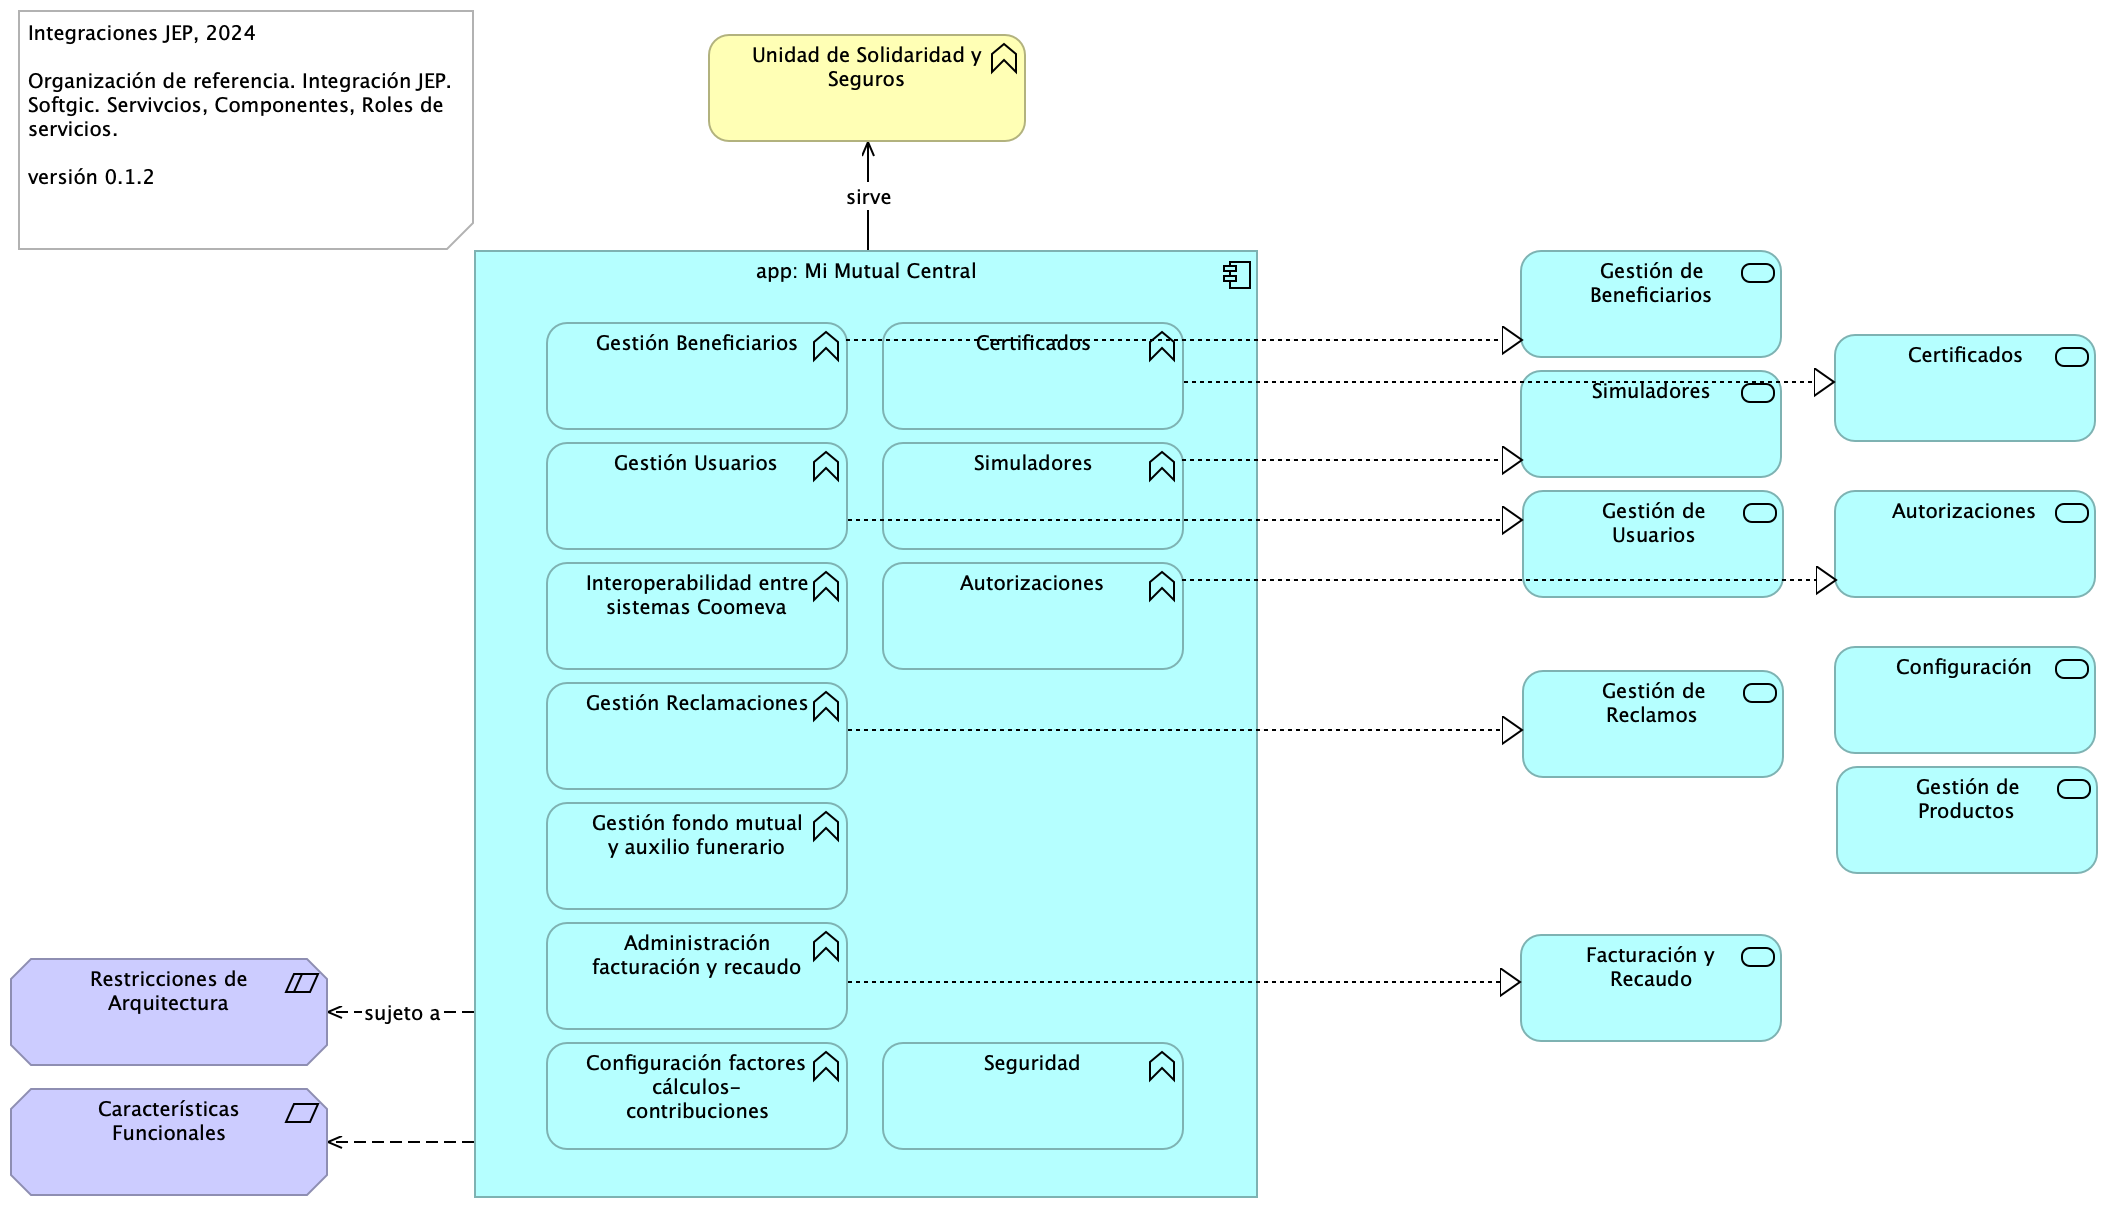
\includegraphics{01.prop.contexto.png}
\caption{1.contexto}
\end{figure}

El sistema principal de fondo Mi Mutual Central es la composición de las
funciones de negocio de la Unidad de Solidaridad de Coomeva. Las
funciones de negocio referidas, como Gestión Beneficiarios,
Certificados, Gestión Beneficiarios, aparecen dentro del componente
principal en la imagen.

Este entregable documenta los diferentes módulos y componentes que hacen
parte de la estructura de una aplicación en Angular 12 y como es su
interacción para conformar una arquitectura robusta y escalable para
aplicaciones de gran tamaño.

Las librerías Spring Boot Security y Spring Boot Oauth2 proveen
características de seguridad entre Vista (Angular 2) y Controlador.
Estas son responsables de que únicamente permita el acceso si se está
autenticado. Además, para realizar el proceso de autenticación se delega
a la aplicación SISPRO (Coomeva) que funciona como un servidor de
autenticación.

\end{document}
